\documentclass[11pt,a4paper]{article}

% AI in Finance course project: edit the four fields below, then body.tex.
\newcommand{\ProjectTitle}{Hybrid Structural and Machine-Learning\\ Corporate Bankruptcy Prediction}
\newcommand{\ProjectAuthors}{Pushkar Gudla (AI24BTECH11012)\\ Vijaya Sreyas Badde (AI24BTECH11003)\\ Adya Thikkavarapu (ES24BTECH11007)}
\newcommand{\CourseName}{AI in Finance}
\newcommand{\CourseTerm}{July--November 2026}

\usepackage[T1]{fontenc}
\usepackage{lmodern}
\usepackage[margin=25mm]{geometry}
\usepackage{microtype}
\usepackage{graphicx}
\usepackage{booktabs}
\usepackage{xcolor}
\usepackage{hyperref}

\definecolor{courseblue}{HTML}{293B87}
\definecolor{promptgray}{HTML}{4D5665}
\hypersetup{
  colorlinks=true,
  linkcolor=courseblue,
  urlcolor=courseblue,
  citecolor=courseblue,
  pdftitle={AI in Finance course project report template},
  pdfauthor={Department of Artificial Intelligence, IIT Hyderabad}
}
\newcommand{\guide}[1]{\par\smallskip\noindent\textcolor{promptgray}{\textbf{Writing guidance.} #1}\par\smallskip}

\begin{document}
\pagenumbering{alph} % unique, unprinted title-page link target
\begin{titlepage}
\centering

\includegraphics[width=3.1cm]{assets/iith-logo.png}\par
\vspace{1.2cm}
{\Large\color{courseblue}\bfseries \CourseName\par}
\vspace{0.25cm}
{\large Course project report \textbar{} \CourseTerm\par}
\vspace{1.55cm}
{\huge\bfseries \ProjectTitle\par}
\vspace{0.9cm}
{\large \ProjectAuthors\par}
\vspace{0.45cm}
{\normalsize Department of Artificial Intelligence\\
Indian Institute of Technology Hyderabad\par}
\vspace{0.5cm}
{\normalsize Submission date: November 2026\par}
\vfill
\begin{minipage}{0.88\textwidth}
\rule{\linewidth}{0.6pt}
\vspace{0.12cm}
{\large\bfseries Abstract}\par\medskip
Lenders and regulators need an early, reliable probability that a firm will fail. We ask whether
the Merton structural credit model adds value to machine-learning (ML) predictors of US corporate
bankruptcy. Using only free SEC EDGAR data, we build a point-in-time panel of 252,943 10-K/10-Q filings
from 10,743 non-financial firms (2010--2025); the target is an 8-K Item~1.03 bankruptcy disclosure within
12 months. Since free price data omit failed firms, we compute an accounting distance to default (DD)
and a public-float naive DD from filings. We compare a structural-only logit, ML models (logit, random
forest, XGBoost, LSTM) and three hybrids on an out-of-time test (2022--2025, 700 positive filings) and
five shift regimes. Gradient-boosted trees with firm history reach AUROC 0.872 versus 0.800 for the
structural model. Structural features improve logistic regression (+0.021 AUROC, firm-bootstrap 95\%
CI [0.013, 0.030]) but not tree models, and give only a modest gain out-of-industry. Qualification:
the structural inputs use book values rather than market prices, and probability levels calibrated on
2020 understate risk in 2022--2025.\par
\vspace{0.12cm}\rule{\linewidth}{0.6pt}
\end{minipage}
\end{titlepage}

\pagenumbering{arabic}
\tableofcontents
\bigskip

% Body of the AI in Finance course project report.
% Hybrid structural and machine-learning corporate bankruptcy prediction.
% Note: the template does not load amsmath, so the maths below uses plain LaTeX only.

\section{Introduction}
\label{sec:introduction}

Banks, bond investors and regulators need a \emph{probability of default} (PD) for every firm they are
exposed to: to price loans, set capital buffers and flag firms for review early. A missed failure costs
the lender most of its exposure; a false alarm costs an unnecessary review or a lost client.

Two traditions produce such PDs. The \textbf{structural} model of Merton~\cite{merton1974} treats equity
as a call option on the firm's assets and turns leverage and asset volatility into one interpretable number,
the \emph{distance to default} (DD). It has almost no free parameters, but rests on strong assumptions and
needs the unobservable asset value and volatility. \textbf{Machine-learning} (ML) models, such as gradient-boosted
trees, learn non-linear patterns from many accounting ratios at once~\cite{moscatelli2020}, but are data-hungry
and may fail when the economy or the population of firms changes.

The prediction is made when a firm files its quarterly (10-Q) or annual (10-K) report, using only what is
public at that moment, and looks 12 months ahead. Three things make it hard: bankruptcy is rare (0.9\% of
filings), bankruptcy rates move with the business cycle, and free price data omit exactly the firms that
fail (delisted stocks disappear), so the market inputs of the Merton model are missing.

\paragraph{Objective.} We test whether structural (Merton) information adds predictive value to ML models,
and whether it helps most where ML is weakest: in a new period, a new industry, for unseen firms, or with
little data. We compare a structural-only model, ML-only models and three hybrids under identical training,
tuning and calibration, on a held-out 2022--2025 test period and five stress tests.

\paragraph{Contributions.}
\begin{enumerate}
  \item A public, point-in-time US bankruptcy panel built only from free SEC EDGAR data: 252,943 filings,
        10,743 firms, 2010--2025, with audited bankruptcy labels and reproducible scripts~\cite{repo}.
  \item Merton features without stock prices: an accounting DD and a public-float naive DD computed from
        filing data, plus a market-data Merton solver for when prices are available.
  \item A controlled comparison of structural, ML and hybrid models, including a control that separates the
        DD formula from its raw inputs, evaluated out-of-time, out-of-industry, on unseen firms, with
        limited data and at three horizons, with firm-cluster confidence intervals.
\end{enumerate}
Section~\ref{sec:problem} defines the task, Section~\ref{sec:methodology} the data and models,
Section~\ref{sec:results} the results and Section~\ref{sec:conclusion} the conclusions and limitations.

\subsection{Related work}
\label{sec:related}

\paragraph{Structural models.} Merton~\cite{merton1974} models firm assets $V_A$ as a geometric Brownian
motion and debt as one zero-coupon bond with face value $D$ due at $T$. Equity is then a European call on
the assets, and default occurs if $V_A(T)<D$. The PD depends only on leverage, asset volatility and horizon.
Bharath and Shumway~\cite{bharath2008} test the KMV implementation of this model on US firms (1980--2003).
A ``naive'' DD that skips the iterative solution ranks firms as well as the full model, so the
\emph{functional form} carries most of the value. They also find that DD is \emph{not} a sufficient
statistic: past returns, profitability and size still add information. Campbell et al.~\cite{campbell2008}
reach a similar conclusion: a reduced-form model with accounting and market variables beats DD.

\paragraph{Machine learning.} Moscatelli et al.~\cite{moscatelli2020} compare logit and discriminant
analysis with random forests and gradient-boosted trees on about 250,000 Italian firm-years (2011--2017).
With public financial data only, trees beat logit by about 2.6 AUROC points; with confidential credit
data the gain shrinks. They also propose downsampling with a Bayes correction for rare defaults and a
PD-bucket backtest. Pellegrino et al.~\cite{pellegrino2024} use 18 annual accounting variables for 8,262 US
firms (1999--2018); a multi-head LSTM reaches a validation AUC of 0.813 versus 0.750 for a random forest.
Their tree baselines, however, see only raw yearly levels, not changes or trends.

\paragraph{Gap.} No study above compares structural, ML and hybrid models side by side under distribution
shift, with a control for ``more variables'', and with a history-aware tree baseline.
Table~\ref{tab:prior-work} summarises the closest studies.

\begin{table}[htbp]
\centering
\small
\begin{tabular}{p{.19\linewidth}p{.23\linewidth}p{.23\linewidth}p{.22\linewidth}}
\toprule
Source & Financial task and data & Method and evaluation & Relation to this project \\
\midrule
Merton (1974)~\cite{merton1974} & Pricing of risky corporate debt; theory & Option-pricing model; no empirical test & Source of the DD and our structural score \\
Bharath \& Shumway (2008)~\cite{bharath2008} & US defaults 1980--2003; firm-months with daily prices & Hazard models with KMV and naive DD; out-of-sample decile tests & We use the naive DD form; RQ1 extends ``is DD sufficient?'' to ML \\
Moscatelli et al.\ (2020)~\cite{moscatelli2020} & Italian firms 2011--2017; firm-years; default on bank loans & Logit vs RF/GBT; AUROC, Brier; small-sample test; PD backtest & ML benchmark, imbalance handling, backtest; we use time-ordered instead of random CV \\
Pellegrino et al.\ (2024)~\cite{pellegrino2024} & US firms 1999--2018; Chapter 7/11 filing next year & Multi-head LSTM vs RF/LR; one time split & We add a tree with lag features (XGB-lag) and structural inputs \\
\bottomrule
\end{tabular}
\caption{Closest related studies and how this project relates to each.}
\label{tab:prior-work}
\end{table}

\section{Problem statement}
\label{sec:problem}

\paragraph{Unit, target and horizon.} One observation is a 10-K or 10-Q filing $i$ of firm $f(i)$, made
public at date $t_i$. The data are $D=\{(x_i, s_i, y_i, t_i)\}_{i=1}^{n}$, where $x_i$ are accounting and
filing features and $s_i$ are structural (Merton) features, all observable at $t_i$. The target is
\begin{equation}
  y_i = \mathbf{1}\{\mbox{the firm's first 8-K Item 1.03 is filed in } (t_i,\; t_i + 12 \mbox{ months}]\}.
  \label{eq:target}
\end{equation}
Item~1.03 of Form~8-K (``Bankruptcy or receivership'') is the firm's own SEC disclosure of a bankruptcy
filing~\cite{sec8k}. The system outputs a calibrated PD $\hat p_i \in [0,1]$ for every filing.

\paragraph{Compared predictors.} With $\sigma(z)=1/(1+e^{-z})$ and $x_i^{(L)}$ the features of the last $L$ filings
($L=1$: a single snapshot),
\begin{equation}
  p_{\mathrm{struct}} = \sigma\left(a + b^{\top} s_i\right), \qquad
  p_{\mathrm{ML}} = g_{\theta}\left(x_i^{(L)}\right), \qquad
  p_{\mathrm{hyb}} = h_{\phi}\left(x_i^{(L)}, s_i^{(L)}\right).
  \label{eq:predictors}
\end{equation}
The \textbf{baseline} for each question is the structural logit $p_{\mathrm{struct}}$ (economic model) and
the same ML model without structural features (``ML-only''). The quantity of interest is
$\Delta = M(p_{\mathrm{hyb}}) - M(p_{\mathrm{ML}})$ for a metric $M$, measured per evaluation regime.

\paragraph{Research questions.}
\begin{description}
  \item[RQ1] Do structural variables add predictive value once flexible accounting and market features are included ($\Delta>0$)?
  \item[RQ2] Are they more useful under distribution shift (new period, new industry, unseen firms) or with limited data ($\Delta$ larger there than out-of-time)?
  \item[RQ3] How sensitive are the results to how the unobservable asset value $V_A$ and volatility $\sigma_A$ are estimated?
  \item[RQ4] Does firm history (lag features or an LSTM) help beyond a single filing, and does structure still help once history is included?
\end{description}

\paragraph{Metrics.} The task is to \emph{rank} firms by risk and to give usable PD levels. Let $\pi$ be
the share of positives in the test set (1.13\%). Higher is better for the first four, lower for Brier.
\begin{itemize}
  \item \textbf{AUROC} (primary): $\Pr(\hat p_i > \hat p_j \mid y_i=1,\, y_j=0)$, the chance that a random
        bankrupt filing is ranked above a random healthy one; 0.5 is random.
  \item \textbf{Average precision} (AP): $\sum_k (R_k - R_{k-1})\, P_k$ over thresholds $k$, with
        precision $P_k$ and recall $R_k$. It focuses on the top of the ranking, where rare positives sit.
  \item \textbf{AP lift} $=\mathrm{AP}/\pi$: how many times richer in bankruptcies the model's top picks are than a random pick.
  \item \textbf{Top-10\% capture}: share of all positives found in the 10\% of filings with the highest $\hat p$.
  \item \textbf{Brier score} $=\frac{1}{n}\sum_i (\hat p_i - y_i)^2$ and calibration plots, for PD levels.
\end{itemize}
Accuracy is not used: predicting ``no bankruptcy'' for every filing is 99\% accurate.

\paragraph{Assumptions and scope.} We study US SEC registrants outside finance (SIC 6000--6999 excluded),
2010--2025. Features use only values reported in the filing itself or earlier. The label is a disclosure
proxy: firms that stop filing before disclosing, and out-of-court restructurings, count as non-events.
No trading or lending costs are modelled; the claims are about ranking and PD accuracy only.

\section{Methodology}
\label{sec:methodology}

All choices below (features, models, splits, metrics) were fixed before scoring the test period, with one
exception reported openly in Section~\ref{sec:caveat}: the class-weighting problem was found in an
ablation after the main evaluation.

\subsection{Data and target construction}

\paragraph{Sources.} Everything comes from free SEC EDGAR bulk files~\cite{secedgar} (no API key):
the \emph{Submissions} file (every filing and its 8-K items), the \emph{Financial Statement Data Sets}
(filing metadata) and \emph{Company Facts} (XBRL values, 1.4\,GB). Each value is taken from the same
filing (accession number) and reporting date, so later restatements cannot leak backwards.

\paragraph{Label.} We rebuilt the event list from the Submissions file: 993 non-financial firms filed an
8-K Item~1.03 since 2010, and 778 of them have usable XBRL filings. Each firm's \emph{first} such 8-K is its
event. Filings on or after the event are dropped (firms keep filing during Chapter~11). Filings after
October 2025 are dropped so every label has a full 12-month window.

\paragraph{Sample.} Table~\ref{tab:panel} summarises the final panel; Figure~\ref{fig:data} shows the
bankruptcy rate over time. It moves with the cycle: peaks in 2015 (commodity bust), 2019 and 2023 (rate
rises), lows in 2013 and 2021.

\begin{table}[htbp]
\centering
\small
\begin{tabular}{lrrrrr}
\toprule
Partition & Years & Filings & Firms & Positive filings (firms) & Rate \\
\midrule
Full panel & 2010--2025 & 252,943 & 10,743 & 2,314 (684) & 0.91\% \\
Train & 2010--2018 & 143,577 & 8,578 & 1,249 (386) & 0.87\% \\
Validation & 2020 & 15,061 & 4,146 & 112 (54) & 0.74\% \\
Test & 2022--Oct 2025 & 62,181 & 5,563 & 700 (212) & 1.13\% \\
\bottomrule
\end{tabular}
\caption{Panel and main split. 2019 and 2021 are purge gaps (Section~\ref{sec:split}).}
\label{tab:panel}
\end{table}

\begin{figure}[htbp]
\centering
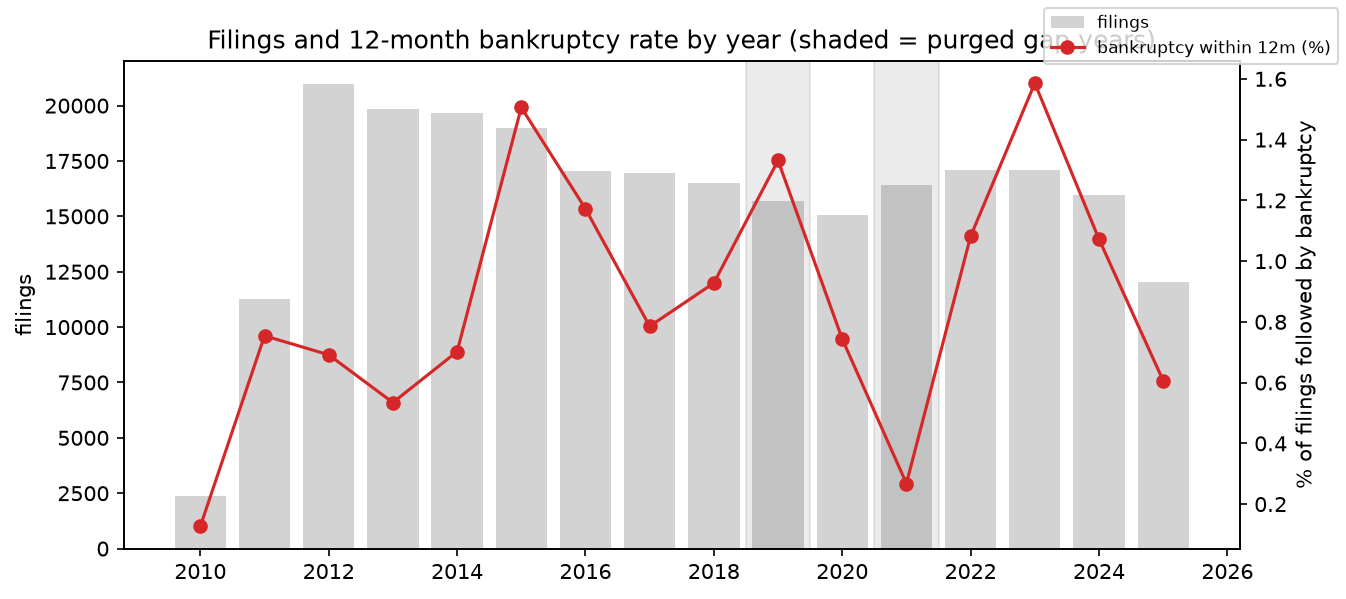
\includegraphics[width=0.8\linewidth]{assets/01_data_by_year.png}
\caption{Filings and share of filings followed by bankruptcy within 12 months, per year. The validation
year 2020 (0.74\%) is calmer than the test years (1.13\%).}
\label{fig:data}
\end{figure}

\paragraph{Features.} Table~\ref{tab:features} lists the feature groups. Quarterly income and cash-flow values
are year-to-date, so they are annualised ($\times 12/\mbox{months}$). Ratios with a denominator below \$1M are
set to missing (shell companies). We drop 130 public-float values dated after their filing and 10,226
implausible ones (zero, above \$5 trillion, or above $10^4\times$ assets).

\begin{table}[htbp]
\centering
\small
\begin{tabular}{p{.22\linewidth}p{.60\linewidth}r}
\toprule
Group & Features & \# \\
\midrule
Balance sheet & liabilities/assets, equity/assets, debt/assets, current ratio, cash/assets, working capital/assets, log assets, \ldots & 10 \\
Income \& cash flow & ROA, EBIT/assets, sales/assets, retained earnings/assets, CFO/assets, interest coverage, loss flag & 7 \\
Cover-page market & log public float, public float/liabilities, float age & 3 \\
Filing metadata & days since previous filing, amendment flag, annual vs quarterly & 3 \\
\midrule
Merton inputs & log default point $D$, asset volatility $\sigma_A$, asset drift $\mu$, equity volatility $\sigma_E$ & 4 \\
Structural outputs & accounting DD, $D/V_A$, public-float naive DD, $E/D$ & 4 \\
\midrule
History (XGB-lag only) & for 12 base ratios: change over 1 and 4 filings; mean, min, max, std and OLS slope over the last 8 filings; number of losses in the last 4 & 85 \\
\bottomrule
\end{tabular}
\caption{Feature groups. Feature set \texttt{ml} = first four groups (23 features); \texttt{hybrid} = all six snapshot groups (31).}
\label{tab:features}
\end{table}

\subsection{Preprocessing and split design}
\label{sec:split}

\paragraph{Preprocessing.} All transformations are fitted on training rows only and then applied to
validation and test rows: clipping to the 1st--99th percentile, median imputation plus a missing-value
indicator, and standardisation (logit, LSTM). XGBoost receives the raw values and handles missing values natively.

\paragraph{Class imbalance.} By default each positive gets weight $w_1 = n_0/n_1 \approx 115$ (negatives 1).
As an ablation we instead keep all positives and a random share $\beta$ of negatives (1:1), then undo the
sampling with the Bayes correction of~\cite{moscatelli2020}:
\begin{equation}
  p = \frac{\beta\, p_s}{\beta\, p_s - p_s + 1},
  \label{eq:bayes}
\end{equation}
where $p_s$ is the score of the model trained on the sample.

\paragraph{Main split (out-of-time).} Train 2010--2018, validation 2020, test January 2022 to October 2025.
The years 2019 and 2021 are \emph{purge gaps}: a filing in December 2018 has a label window that runs to
December 2019, so without the gap its outcome would overlap the next partition. The validation year is
used only for probability calibration, LSTM early stopping and fitting the stacking model, never to pick
models by test score.

\paragraph{Firms across partitions.} A firm can appear in train and test (at different times), as it would
in deployment. A separate \emph{unseen-firms} regime removes 30\% of firms from training entirely.
Because one firm has about four filings a year with correlated outcomes, all uncertainty estimates resample
\emph{firms}, not filings (Section~\ref{sec:metrics}).

\subsection{Models, baselines, and tuning}
\label{sec:models}

\paragraph{Merton model.} With risk-free rate $r$ and standard normal CDF $\Phi$, equity is a call on assets:
\begin{equation}
  E = V_A \Phi(d_1) - D e^{-rT}\Phi(d_2), \qquad
  d_1 = \frac{\ln(V_A/D) + (r + \frac{1}{2}\sigma_A^2)T}{\sigma_A\sqrt{T}}, \qquad d_2 = d_1 - \sigma_A\sqrt{T},
  \label{eq:merton}
\end{equation}
and It\^o's lemma links equity and asset volatility, $\sigma_E E = \Phi(d_1)\,\sigma_A V_A$. Given $E$ and
$\sigma_E$ from stock prices, these two equations are solved for $(V_A,\sigma_A)$, and
\begin{equation}
  \mathrm{DD} = \frac{\ln(V_A/D) + (\mu - \frac{1}{2}\sigma_A^2)T}{\sigma_A\sqrt{T}}, \qquad \mathrm{PD} = \Phi(-\mathrm{DD}).
  \label{eq:dd}
\end{equation}
Our solver reduces the 2-D system to nested 1-D bisections on the brackets
$V_A \in [E,\, E + De^{-rT}]$ and $\sigma_A \in [\sigma_E E/(E+De^{-rT}),\, \sigma_E]$, so it always converges,
and implements the four DD variants of~\cite{bharath2008}. It needs daily prices, which free sources provide
for only 29 of 489 bankrupt firms in our first (Yahoo) panel. We therefore built two price-free versions.

\paragraph{Accounting DD.} Keep the form of~(\ref{eq:dd}) with $T=1$ and replace market inputs by filing data,
as in Moody's KMV private-firm model:
$V$ = book total assets; default point $D = \mathrm{CL} + \frac{1}{2}(\mathrm{L}-\mathrm{CL})$ with current
liabilities CL and total liabilities L (92\% coverage, against 50\% for a debt-based point); $\mu$ = trailing
asset growth, clipped to $\pm 50\%$. Asset volatility comes from the firm's last $n\le 9$ filings with
irregular gaps $\Delta t_k$, shrunk towards the median $\bar\sigma_{\mathrm{SIC2}}$ of its industry (training years only):
\begin{equation}
  \hat\sigma^2 = \frac{n}{n-1}\cdot\frac{\sum_k (\Delta_k \ln V - \hat\mu\,\Delta t_k)^2}{\sum_k \Delta t_k},
  \qquad
  \sigma_A = \max\left(\frac{n}{n+4}\,\hat\sigma + \frac{4}{n+4}\,\bar\sigma_{\mathrm{SIC2}},\; 0.05\right).
  \label{eq:sigma}
\end{equation}

\paragraph{Public-float naive DD.} Each 10-K cover page reports the \emph{public float}, the market value of
equity held by non-insiders: a real market price, but only once a year. With $E$ = latest float, $\sigma_E$
from float-implied price changes (up to six years, shrunk to the industry median), $\mu$ = past-year
float-implied return and the same $D$, the naive formula of~\cite{bharath2008} gives
\begin{equation}
  V = E + D,\quad \sigma_D = 0.05 + 0.25\,\sigma_E,\quad
  \sigma_V = \frac{E}{V}\sigma_E + \frac{D}{V}\sigma_D,\quad
  \mathrm{DD}^{\mathrm{pf}} = \frac{\ln(V/D) + \mu - \frac{1}{2}\sigma_V^2}{\sigma_V}.
  \label{eq:naive}
\end{equation}

\paragraph{Structural baseline.} The structural model is the logit $p_{\mathrm{struct}}=\sigma(a+b^\top s)$
on four structural outputs: accounting DD, $D/V_A$, public-float DD and $E/D$.

\paragraph{ML models.} All use the \texttt{ml} features (Table~\ref{tab:features}).
\begin{itemize}
  \item \textbf{Logistic regression} with L2 penalty (statistical benchmark, as in~\cite{moscatelli2020}).
  \item \textbf{Random forest}: 500 trees, minimum leaf 20, $\sqrt{p}$ features per split.
  \item \textbf{XGB-static}~\cite{chen2016xgboost}: gradient-boosted trees on one filing; 500 trees, depth 4,
        learning rate 0.03, subsample and column sample 0.8, minimum child weight 5.
  \item \textbf{XGB-lag}: XGB-static plus the 85 history features: a history-aware tree baseline.
  \item \textbf{LSTM}~\cite{hochreiter1997lstm} over the last 8 filings: 2 layers, 64 units, dropout 0.25,
        AdamW (learning rate $5\cdot10^{-4}$, weight decay $10^{-3}$), batch 512, up to 30 epochs with early
        stopping on validation AP (patience 5), average of 3 seeds. Firms with fewer than 8 past filings are
        zero-padded with a padding flag, so the LSTM scores exactly the same rows as the trees.
\end{itemize}

\paragraph{Hybrid models.}
\begin{itemize}
  \item \textbf{H1, structure as features:} the same model on the \texttt{hybrid} set. To test whether a gain
        comes from the DD \emph{formula} or just from extra inputs, a \textbf{control} model uses
        \texttt{ml} + Merton inputs ($D,\sigma_A,\mu,\sigma_E$) but no DD outputs (Bharath and Shumway's question).
  \item \textbf{H2, structure as a prior:} the structural logit is fitted first and the ML model learns only a correction,
        \begin{equation}
          \mathrm{logit}\, p_{\mathrm{H2}}(x) = \underbrace{a + b^\top s}_{\mbox{\scriptsize fixed structural prior}} + \underbrace{f_\theta(x)}_{\mbox{\scriptsize learned correction}}.
          \label{eq:h2}
        \end{equation}
        In XGBoost the prior is the starting margin (\texttt{base\_margin}); in the LSTM it is added to the output.
        With little or unfamiliar data, $f_\theta\approx 0$ and the model falls back to the economic PD. H2 is
        trained without class weights, since the prior is already on the population scale.
  \item \textbf{H3, stacking:} a logistic model on the log-odds of the structural, XGB-lag and LSTM predictions,
        fitted on the 2020 validation year:
        $\mathrm{logit}\, p_{\mathrm{H3}} = c_0 + c_1\,\mathrm{logit}\, p_{\mathrm{struct}} + c_2\,\mathrm{logit}\, p_{\mathrm{XGB\mbox{-}lag}} + c_3\,\mathrm{logit}\, p_{\mathrm{LSTM}}$.
\end{itemize}

\paragraph{Calibration.} Raw scores are mapped to PDs by Platt scaling~\cite{platt1999}, fitted on the 2020
validation year and then applied unchanged to the test set:
\begin{equation}
  \hat p = \sigma\left(\alpha\,\mathrm{logit}(p_{\mathrm{raw}}) + \gamma\right).
  \label{eq:platt}
\end{equation}
The map is monotone, so it changes PD levels but never the ranking (AUROC). Isotonic regression was tested as an alternative.

\paragraph{Tuning.} Each model family gets the same budget: 4 random-search trials, the first being the
default setting above. A trial is scored by mean AP over four time-ordered folds inside the training years
(fit on years $\le Y-2$, score year $Y$, $Y=2015,\ldots,2018$). Random $k$-fold CV, as used
in~\cite{moscatelli2020}, would leak here because the same firm sits in many folds and neighbouring filings
share an outcome window. Each family is tuned on \texttt{ml} and the parameters are reused for its hybrid, which
is conservative for the hybrid. Search spaces: logit $C\in\{10^{-4},\ldots,10\}$; random forest depth
$\{\mbox{none},8,12,16\}$, minimum leaf $\{5,20,50,100\}$, features $\{\sqrt{p},0.3,0.5\}$; XGBoost trees
$\{300,500,800\}$, learning rate $\{0.01,0.03,0.05,0.1\}$, depth $\{3,\ldots,6\}$, minimum child weight
$\{1,5,20\}$, subsample and column sample $\{0.5\mbox{--}1.0\}$, L2 penalty $\{1,5,20\}$. The logit chose
$C=0.001$; for the random forest and XGBoost the defaults won. The LSTM used fixed defaults.

\paragraph{Software.} Python with NumPy, pandas, scikit-learn ($\ge$1.3), XGBoost ($\ge$2.0, \texttt{hist} trees)
and PyTorch ($\ge$2.2). Seeds: 42 for the forest and XGBoost, 0 for tuning and bootstrap, 0--2 for the LSTM.

\subsection{Experiments and metrics}
\label{sec:metrics}

Table~\ref{tab:regimes} maps each experiment to its question. The structural-prior hypothesis (RQ2)
predicts that $\Delta$ is larger in the stress tests than in the main split.

\begin{table}[htbp]
\centering
\small
\begin{tabular}{p{.20\linewidth}p{.45\linewidth}p{.25\linewidth}}
\toprule
Regime & What is held out & Question \\
\midrule
Main (out-of-time) & train 2010--18, test 2022--25 & RQ1, RQ4 \\
Rolling years & for each test year $T$ (2015--2025): train $\le T-4$, validate $T-2$, test $T$ & stability over time (RQ2) \\
Out-of-industry & one SIC division with $\ge$20 bankrupt firms; train on the others; test on it in 2010--18 (and in 2022--25) & new industry (RQ2) \\
Unseen firms & 30\% of firms removed from training and validation; 3 random draws & new companies (RQ2) \\
Limited data & train on 2--100\% of training firms; 5 draws (skipped if $<$10 bankrupt firms) & little data (RQ2) \\
Horizon & label window of 3, 6 or 12 months & close to the event (RQ2) \\
Ablations & feature groups; DD variants; class weights; calibration; LSTM window & RQ1, RQ3 \\
\bottomrule
\end{tabular}
\caption{Evaluation regimes.}
\label{tab:regimes}
\end{table}

\paragraph{Uncertainty.} For a difference $\Delta = M(p_a)-M(p_b)$ on the same test rows we draw 500
bootstrap samples of \emph{firms} with replacement (keeping all filings of a drawn firm), recompute $\Delta$,
and report the 2.5\% and 97.5\% percentiles as a 95\% confidence interval. A difference is called significant
when the interval excludes zero. Repeated regimes (unseen firms, limited data) report the mean and standard
deviation over draws.

\paragraph{Interpretation.} Three views per feature group of the hybrid XGBoost: (i) share of mean absolute
SHAP value~\cite{lundberg2017shap} (how much the model \emph{uses} the group); (ii) AUROC drop when the group
is shuffled in the trained model (how much it \emph{relies} on it); (iii) AUROC drop when the model is
retrained without it (whether other features can \emph{replace} it).

\paragraph{PD backtest.} Following~\cite{moscatelli2020}, test filings are grouped into PD buckets. In a bucket
with $n$ filings, $k$ bankruptcies and upper PD bound $\bar p$, the p-value is $\Pr(X\ge k)$ with
$X\sim\mathrm{Binomial}(n,\bar p)$; the bucket is red if $p<0.01$, yellow if $p<0.10$, green otherwise.

\section{Results and analysis}
\label{sec:results}

\subsection{Main comparison (out-of-time, 2022--2025)}

\begin{table}[htbp]
\centering
\small
\begin{tabular}{llcccc}
\toprule
Family & Model & AUROC & AP & AP lift & Top-10\% capture \\
\midrule
Structural & Structural logit (baseline) & 0.800 & 0.041 & 3.6$\times$ & 44.9\% \\
\midrule
Statistical & Logit, \texttt{ml} & 0.827 & 0.051 & 4.6$\times$ & 45.1\% \\
            & Logit, \texttt{hybrid} (H1) & 0.848 & 0.064 & 5.7$\times$ & 52.0\% \\
\midrule
Trees & Random forest, \texttt{ml} & 0.862 & 0.086 & 7.6$\times$ & 55.3\% \\
      & Random forest, \texttt{hybrid} (H1) & 0.864 & 0.098 & 8.7$\times$ & 56.9\% \\
      & XGB-static, \texttt{ml} & 0.862 & 0.088 & 7.9$\times$ & 58.6\% \\
      & XGB-static, control (Merton inputs) & 0.859 & 0.091 & 8.0$\times$ & 54.7\% \\
      & XGB-static, \texttt{hybrid} (H1) & 0.855 & 0.087 & 7.8$\times$ & 54.7\% \\
      & XGB-static + prior (H2) & 0.865 & 0.093 & 8.3$\times$ & 59.9\% \\
\midrule
History & XGB-lag, \texttt{ml} & \textbf{0.872} & 0.100 & 8.9$\times$ & 59.1\% \\
        & XGB-lag, \texttt{hybrid} (H1) & 0.869 & 0.096 & 8.6$\times$ & 59.0\% \\
        & LSTM, \texttt{ml} & 0.854 & 0.068 & 6.0$\times$ & 52.1\% \\
        & LSTM, \texttt{hybrid} (H1) & 0.843 & 0.076 & 6.7$\times$ & 53.3\% \\
\midrule
Stacking & Structural + XGB-lag + LSTM (H3) & \textbf{0.872} & \textbf{0.103} & \textbf{9.2}$\times$ & 58.7\% \\
\bottomrule
\end{tabular}
\caption{Held-out test 2022--October 2025: 62,181 filings, 700 positive filings from 212 firms (base rate
$\pi$ = 1.13\%). Higher is better for all columns. All models calibrated on 2020.}
\label{tab:results}
\end{table}

Table~\ref{tab:results} gives the main result. Every ML model beats the structural baseline: XGB-static by
+0.062 AUROC (95\% CI [0.039, 0.084]). Trees beat the logit by +0.035 [0.021, 0.047], close to the 2.6 points
reported by~\cite{moscatelli2020} on public data. The best single model is XGB-lag (AUROC 0.872, AP lift
8.9$\times$); stacking matches its AUROC with the highest AP (9.2$\times$ the base rate). The best models place
about 59\% of all bankruptcies in their riskiest 10\% of filings. Figure~\ref{fig:roc} shows that the ML
curves lie above the structural one along the whole ROC curve, and that precision stays low in absolute
terms: about 10\% at 40\% recall, still roughly 9 times the base rate.

\begin{figure}[htbp]
\centering
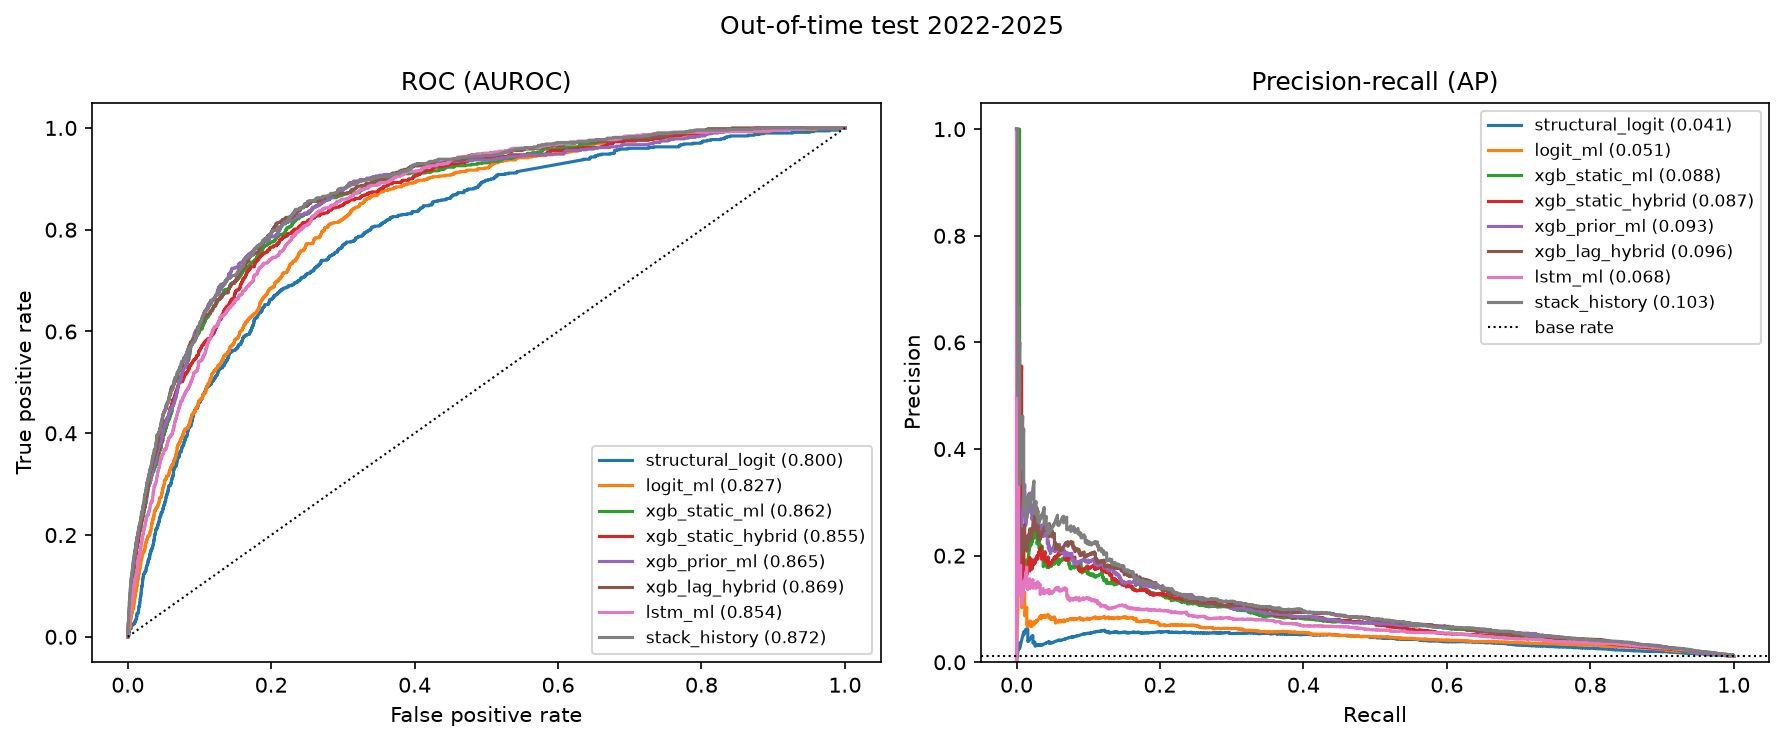
\includegraphics[width=0.95\linewidth]{assets/06_roc_pr.png}
\caption{ROC (left) and precision--recall (right) curves on the 2022--2025 test set; the AUROC or AP of each model is in the legend.}
\label{fig:roc}
\end{figure}

\subsection{RQ1 and RQ4: does structure help, and does history help?}

\begin{table}[htbp]
\centering
\small
\begin{tabular}{lcc}
\toprule
Comparison (A $-$ B) & $\Delta$ AUROC [95\% CI] & $\Delta$ AP [95\% CI] \\
\midrule
\multicolumn{3}{l}{\emph{Structure (RQ1)}} \\
Logit: hybrid $-$ ml & \textbf{+0.021} [0.013, 0.030] & \textbf{+0.013} [0.007, 0.020] \\
Random forest: hybrid $-$ ml & +0.003 [$-$0.002, 0.008] & +0.012 [$-$0.001, 0.025] \\
XGB-static: hybrid $-$ ml & $-$0.007 [$-$0.014, 0.001] & $-$0.001 [$-$0.013, 0.013] \\
XGB-static: hybrid $-$ control (DD formula) & $-$0.003 [$-$0.008, 0.000] & $-$0.003 [$-$0.012, 0.005] \\
XGB-static: prior (H2) $-$ ml & +0.003 [$-$0.006, 0.012] & +0.005 [$-$0.007, 0.018] \\
XGB-lag: hybrid $-$ ml & $-$0.002 [$-$0.006, 0.002] & $-$0.004 [$-$0.020, 0.008] \\
\midrule
\multicolumn{3}{l}{\emph{History (RQ4)}} \\
XGB-lag $-$ XGB-static (ml) & \textbf{+0.010} [0.001, 0.020] & +0.011 [$-$0.003, 0.033] \\
LSTM $-$ XGB-lag (ml) & \textbf{$-$0.018} [$-$0.032, $-$0.004] & \textbf{$-$0.032} [$-$0.058, $-$0.013] \\
\midrule
\multicolumn{3}{l}{\emph{Models}} \\
XGB-static $-$ logit (ml) & \textbf{+0.035} [0.021, 0.047] & \textbf{+0.037} [0.018, 0.060] \\
\bottomrule
\end{tabular}
\caption{Paired differences on the test set with firm-bootstrap 95\% CIs (500 resamples). Bold: CI excludes zero.}
\label{tab:deltas}
\end{table}

\paragraph{Structure (RQ1).} Table~\ref{tab:deltas} shows that structural features clearly help the
\emph{linear} model (+0.021 AUROC). For every tree model the difference is within $\pm$0.007 and every
interval contains zero. The control answers Bharath and Shumway's question for trees: given the raw Merton
inputs, adding the DD formula itself changes AUROC by $-0.003$. A plausible reason for the logit gain is that
a logit can only use each input linearly, while DD is a non-linear combination of leverage and volatility
that trees can build themselves.

\paragraph{History (RQ4).} Lag features help trees (+0.010 AUROC). The LSTM, which must learn its own history
features, is clearly worse than XGB-lag ($-0.018$ AUROC, $-0.032$ AP), and adding structure to a model
that already has history changes nothing.

\paragraph{Why does structure not help the trees?} Figure~\ref{fig:shap} shows that the hybrid XGBoost does
\emph{use} structural information: 26\% of the total SHAP attribution (Merton inputs 16\%, DD outputs 10\%),
with asset growth $\mu$ and the default point among its seven most-used features. Table~\ref{tab:ablation}
shows that it does not \emph{need} it: shuffling the structural groups costs little, and retraining without
them costs nothing (the last row is exactly the control model). The trees rebuild the same signal from
leverage, profitability and size. Only the income and cash-flow ratios cannot be replaced ($-0.032$ AUROC),
in line with~\cite{bharath2008,campbell2008}.

\begin{figure}[htbp]
\centering
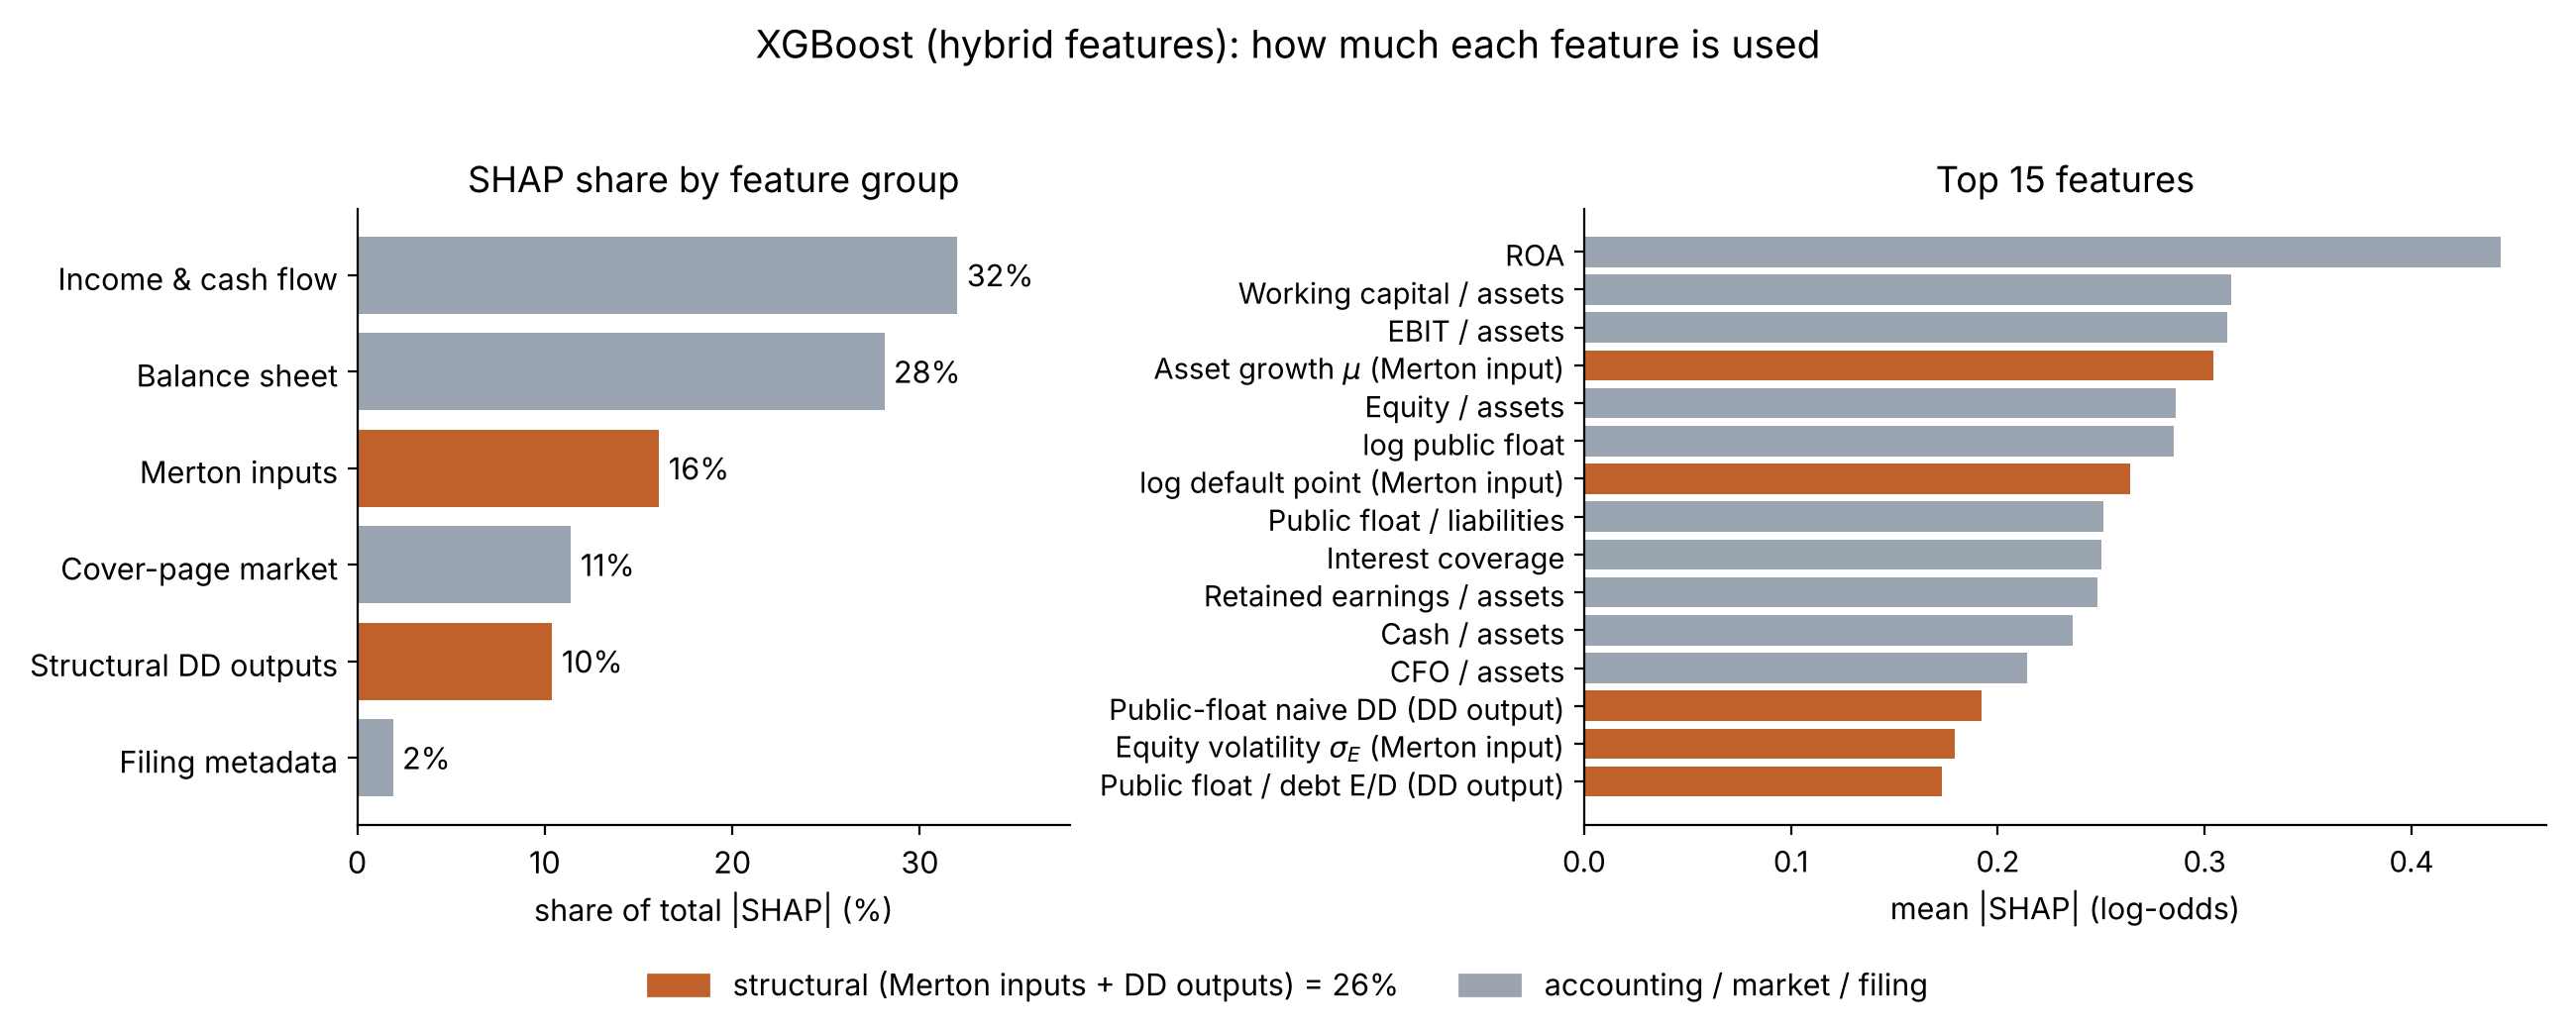
\includegraphics[width=\linewidth]{assets/07_shap_groups_structural.png}
\caption{Mean absolute SHAP values of the hybrid XGB-static, by feature group (left) and for the
top 15 features (right). Orange: structural features.}
\label{fig:shap}
\end{figure}

\begin{table}[htbp]
\centering
\small
\begin{tabular}{lccc}
\toprule
Feature group & SHAP share & Shuffle: AUROC drop & Remove and retrain: AUROC drop \\
\midrule
Income \& cash flow & 32\% & 0.138 & \textbf{0.032} \\
Balance sheet & 28\% & 0.076 & 0.008 \\
Merton inputs & 16\% & 0.023 & $-$0.004 \\
Cover-page market & 11\% & 0.009 & $-$0.003 \\
Structural DD outputs & 10\% & 0.004 & $-$0.003 \\
Filing metadata & 2\% & 0.000 & 0.000 \\
\bottomrule
\end{tabular}
\caption{Three views of each feature group in the hybrid XGB-static (test AUROC 0.855). Negative drops mean the model improved slightly, within noise.}
\label{tab:ablation}
\end{table}

\subsection{RQ3: sensitivity to the structural construction}

Table~\ref{tab:rq3} scores each structural measure alone (one-variable logit, same test set). The choice of
\emph{default point} matters far more than the drift: a debt-based point loses coverage (49\%, because debt
tags are often missing) and ranks much worse (0.644), while dropping the drift costs 0.024 AUROC and
leaves the ranking almost unchanged (rank correlation 0.985 with the main DD). The full DD beats leverage
$D/V_A$ alone, so volatility and drift add information. The public-float DD is weaker (0.693): it is a true
market price but up to 15 months old. Inside the hybrid XGBoost, the choice of variant changes AUROC by at most
0.003 (0.854--0.858), so RQ1 does not depend on it. The comparison of iterative and naive market DDs
of~\cite{bharath2008} could not be run at scale, because it needs daily prices for failed firms.

\begin{table}[htbp]
\centering
\small
\begin{tabular}{lcccc}
\toprule
Structural measure & AUROC & AP & AP lift & Test coverage \\
\midrule
Accounting DD (main) & \textbf{0.791} & \textbf{0.040} & 3.5$\times$ & 85\% \\
\quad no drift ($\mu=0$) & 0.767 & 0.033 & 2.9$\times$ & 85\% \\
\quad debt-based default point & 0.644 & 0.029 & 2.5$\times$ & 49\% \\
Default point / assets ($D/V_A$) only & 0.769 & 0.034 & 3.1$\times$ & 85\% \\
Public-float naive DD & 0.693 & 0.029 & 2.6$\times$ & 86\% \\
\midrule
All four structural outputs (structural logit) & 0.800 & 0.041 & 3.6$\times$ & -- \\
\bottomrule
\end{tabular}
\caption{Each structural measure alone in a one-variable logit, test 2022--2025.}
\label{tab:rq3}
\end{table}

Figure~\ref{fig:event} shows how the signals evolve before bankruptcy: the accounting DD stays flat (about
2.8) until roughly 20 months before the event and then falls below zero, while the public-float DD declines
steadily over three years: market prices react earlier than balance sheets.

\begin{figure}[htbp]
\centering
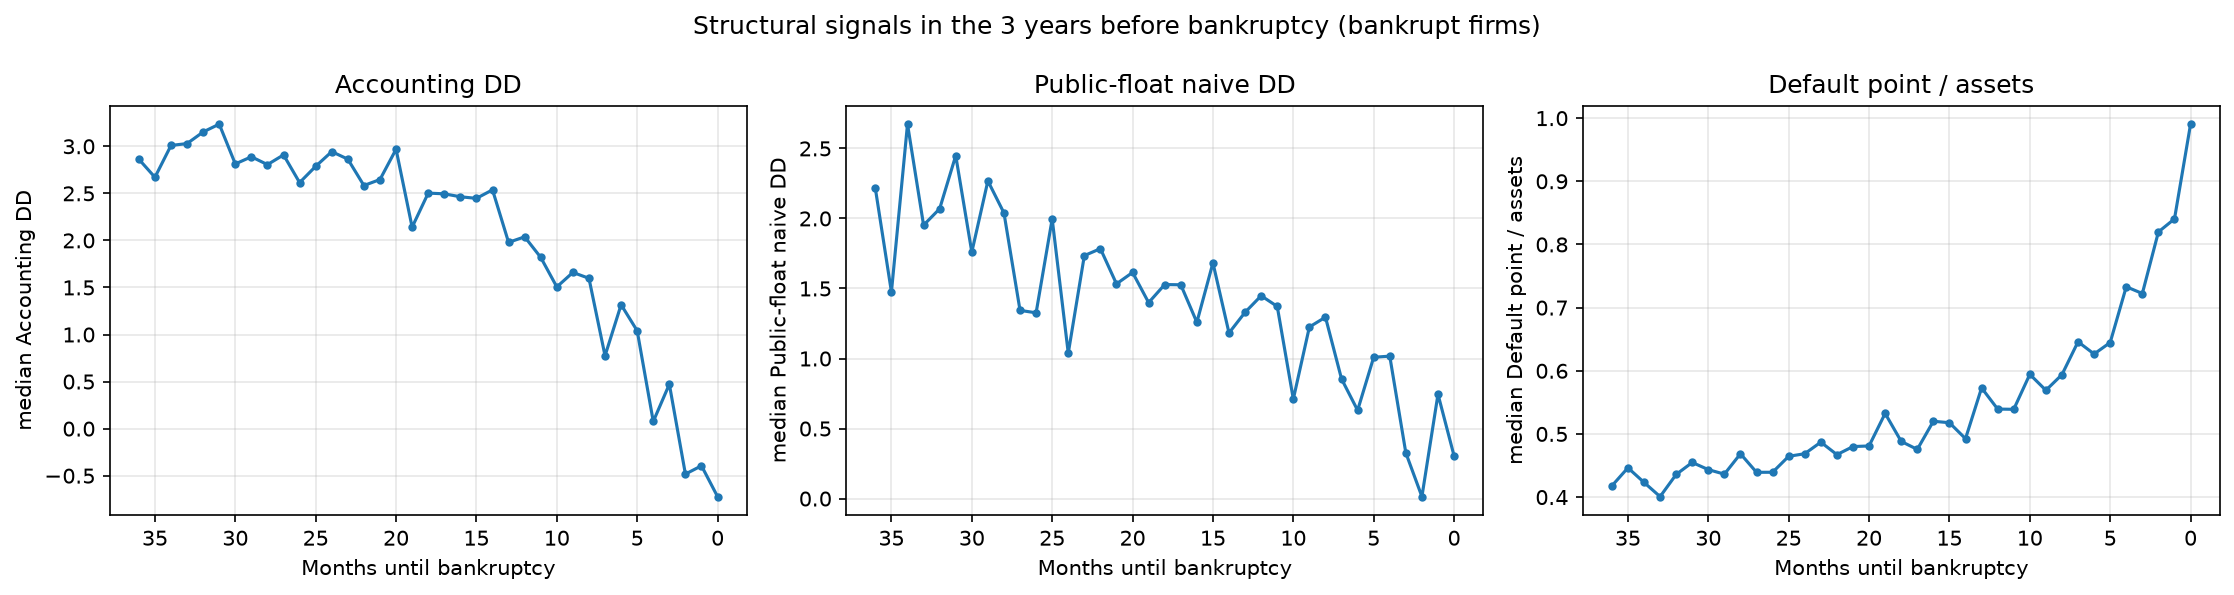
\includegraphics[width=0.9\linewidth]{assets/02_dd_before_bankruptcy.png}
\caption{Median structural signals of bankrupt firms by months until the bankruptcy disclosure.}
\label{fig:event}
\end{figure}

\subsection{RQ2: distribution shift and limited data}

\paragraph{New industry.} Holding out one SIC division (Table~\ref{tab:ooi}), H1 beats ML in 4 of 6
industries on both AUROC and AP lift, and raises the mean AUROC from 0.839 to 0.847: a modest tilt, unlike
the zero effect out-of-time. The large average gain in AP lift is driven by Retail, which has only 30
positives. When the industry \emph{and} the period are both new, the gain disappears (mean AUROC: ML 0.869,
H1 0.867, H2 0.867). H2 is clearly worse in Mining (0.782), where a prior fitted on other industries points
the wrong way.

\begin{table}[htbp]
\centering
\small
\begin{tabular}{lrcccc}
\toprule
Held-out division & Positives & Structural & ML (XGB) & H1 hybrid & H2 prior \\
\midrule
Manufacturing & 409 & 0.787 / 3.9$\times$ & 0.853 / 7.8$\times$ & \textbf{0.864} / 8.8$\times$ & 0.853 / \textbf{8.8$\times$} \\
Mining & 416 & 0.703 / 2.4$\times$ & 0.820 / 7.6$\times$ & \textbf{0.855} / \textbf{8.3$\times$} & 0.782 / 8.2$\times$ \\
Services & 158 & 0.746 / 3.9$\times$ & 0.779 / \textbf{10.7$\times$} & 0.777 / 8.9$\times$ & \textbf{0.803} / 10.3$\times$ \\
Transport \& utilities & 181 & 0.712 / 3.2$\times$ & \textbf{0.828} / 6.1$\times$ & 0.819 / 7.4$\times$ & 0.806 / \textbf{9.8$\times$} \\
Wholesale & 50 & 0.755 / 3.3$\times$ & 0.807 / \textbf{17.2$\times$} & 0.820 / 15.3$\times$ & \textbf{0.824} / 14.0$\times$ \\
Retail & 30 & 0.942 / 18.6$\times$ & 0.943 / 21.1$\times$ & 0.948 / 40.7$\times$ & \textbf{0.971} / \textbf{46.2$\times$} \\
\midrule
Mean & & 0.774 / 5.9$\times$ & 0.839 / 11.8$\times$ & \textbf{0.847} / 14.9$\times$ & 0.840 / \textbf{16.2$\times$} \\
\bottomrule
\end{tabular}
\caption{Out-of-industry test (training years 2010--2018). Cells: AUROC / AP lift.}
\label{tab:ooi}
\end{table}

\paragraph{Unseen firms and stability over time.} With 30\% of firms never seen in training (3 draws), the
mean AUROC is 0.793 (structural), 0.855 (ML), 0.854 (H1) and 0.865 (H2), and H2 is the most stable
(standard deviation 0.001 against 0.013 for ML). In year-by-year retraining (Figure~\ref{fig:rolling}), ML and
H1 move together and the structural model is last in every year (gap 0.12 in 2015, 0.01 in 2025). All models
dip in 2021, a year with only 23 bankrupt firms. H2 is clearly worse in 2015--2016, when only 2010--2012
data are available for training: the prior did not help when history was short.

\begin{figure}[htbp]
\centering
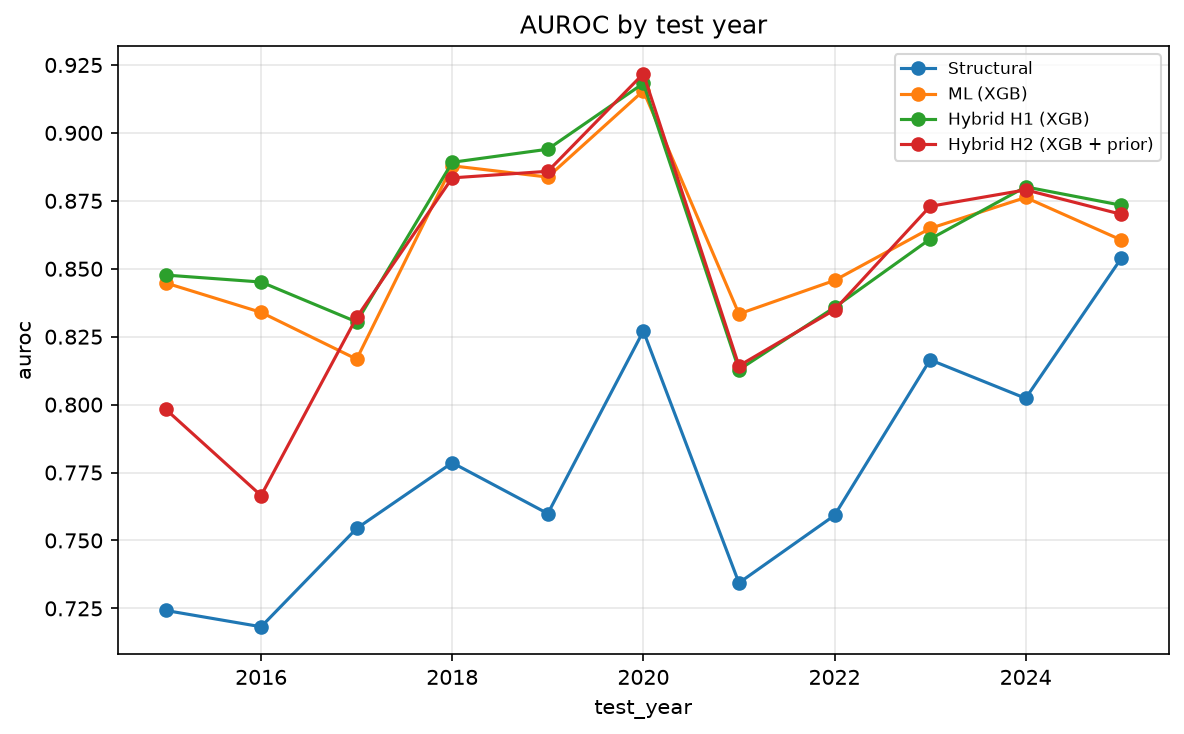
\includegraphics[width=0.75\linewidth]{assets/08_rolling_auroc.png}
\caption{Test AUROC per year with yearly retraining (train $\le T-4$, test $T$).}
\label{fig:rolling}
\end{figure}

\paragraph{Limited data.} Training on a random share of firms (Table~\ref{tab:limited}), the hybrids are not
consistently better than ML at any size; the differences (below 0.01) are within the variation between draws.
Even with about 22 bankrupt training firms XGBoost stays well above the structural model, and the structural model
itself improves with more data (0.76 to 0.80), so it is not a free data-efficient fallback.

\begin{table}[htbp]
\centering
\small
\begin{tabular}{lccccc}
\toprule
Share of training firms & Bankrupt training firms & Structural & ML (XGB) & H1 hybrid & H2 prior \\
\midrule
5\% & 22 & 0.760 & 0.784 & 0.790 & 0.784 \\
10\% & 41 & 0.780 & 0.813 & 0.820 & 0.818 \\
25\% & 97 & 0.790 & 0.835 & 0.831 & 0.837 \\
50\% & 186 & 0.792 & 0.847 & 0.848 & 0.851 \\
100\% & 386 & 0.800 & 0.862 & 0.855 & 0.865 \\
\bottomrule
\end{tabular}
\caption{Test AUROC with limited training data (mean over 5 draws; standard deviations 0.005--0.038; 100\% is a single run).
The 2\% share is omitted: only one of its draws had at least 10 bankrupt firms.}
\label{tab:limited}
\end{table}

\paragraph{Horizon.} Table~\ref{tab:horizon} shows that every model is better closer to the event, and the
structural model gains the most (0.800 to 0.856): DD captures \emph{imminent} distress. H2 has the highest AUROC
at every horizon, but by small margins (0.002--0.011 over the next model).

\begin{table}[htbp]
\centering
\small
\begin{tabular}{lcccccc}
\toprule
 & \multicolumn{2}{c}{3 months} & \multicolumn{2}{c}{6 months} & \multicolumn{2}{c}{12 months} \\
\cmidrule(lr){2-3}\cmidrule(lr){4-5}\cmidrule(lr){6-7}
Model & AUROC & AP lift & AUROC & AP lift & AUROC & AP lift \\
\midrule
Structural & 0.856 & 5.3$\times$ & 0.837 & 4.6$\times$ & 0.800 & 3.6$\times$ \\
ML (XGB) & 0.887 & 13.7$\times$ & 0.881 & 11.7$\times$ & 0.862 & 7.9$\times$ \\
H1 hybrid & 0.895 & 12.5$\times$ & 0.879 & \textbf{12.6$\times$} & 0.855 & 7.8$\times$ \\
H2 prior & \textbf{0.897} & \textbf{14.6$\times$} & \textbf{0.892} & 11.7$\times$ & \textbf{0.865} & \textbf{8.3$\times$} \\
\midrule
Test positives & \multicolumn{2}{c}{139} & \multicolumn{2}{c}{309} & \multicolumn{2}{c}{700} \\
\bottomrule
\end{tabular}
\caption{Test 2022--2025 with label windows of 3, 6 and 12 months.}
\label{tab:horizon}
\end{table}

\subsection{A caveat on H2: class weights}
\label{sec:caveat}

Several H2 results look favourable (main test, unseen firms, horizon). However, an ablation run after the main
evaluation (Table~\ref{tab:imbalance}) shows that XGBoost does \emph{better without} class weights once it is
calibrated: a weight of about 115 makes the trees over-fit the few positives. H2 is trained without weights by
design, while the ML baseline uses them. Part or all of H2's edge may therefore come from dropping the weights,
not from the structural prior. Until H2 is compared with an unweighted ML model, we do not claim that H2 helps.
This does not affect H1 or the history comparisons, where both sides use the same weighting.

\begin{table}[htbp]
\centering
\small
\begin{tabular}{lccc}
\toprule
Imbalance handling (XGB-static, \texttt{hybrid}) & AUROC & AP & Brier \\
\midrule
Class weights $w_1\approx115$ (default) & 0.855 & 0.087 & 0.0107 \\
Downsampling 1:1 + Bayes correction~(\ref{eq:bayes}) & 0.864 & 0.080 & 0.0108 \\
No re-weighting & \textbf{0.868} & \textbf{0.098} & \textbf{0.0107} \\
\bottomrule
\end{tabular}
\caption{Imbalance ablation; all variants Platt-calibrated on 2020.}
\label{tab:imbalance}
\end{table}

\subsection{Calibration and error analysis}

\paragraph{PD levels.} Ranking holds up, but PD levels do not. Without calibration, the class-weighted XGBoost
predicts a mean PD of 18\% against a realised 1.1\% (Brier 0.094); Platt scaling reduces the Brier score to 0.011
(isotonic: 0.011, with a slightly lower AUROC of 0.849). Yet the calibrated mean PD on the test set is 0.77\%
against a realised 1.13\%: the calibrator learned the rate of the calm year 2020 (0.74\%). In the PD-bucket
backtest (Figure~\ref{fig:calibration}), the four low-PD buckets are red, with 2--6 times more bankruptcies than
predicted, and the high-PD buckets are green. This matches the ``slow adaptation'' that~\cite{moscatelli2020}
report during default surges.

\begin{figure}[htbp]
\centering
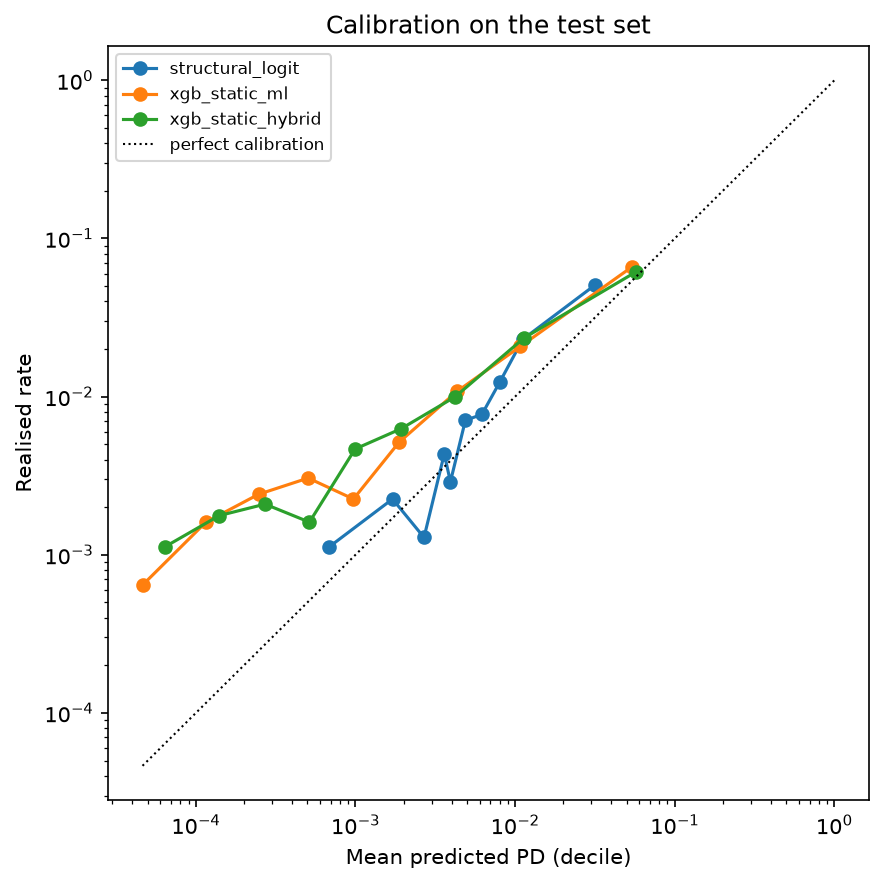
\includegraphics[height=5.6cm]{assets/06_calibration.png}\hfill
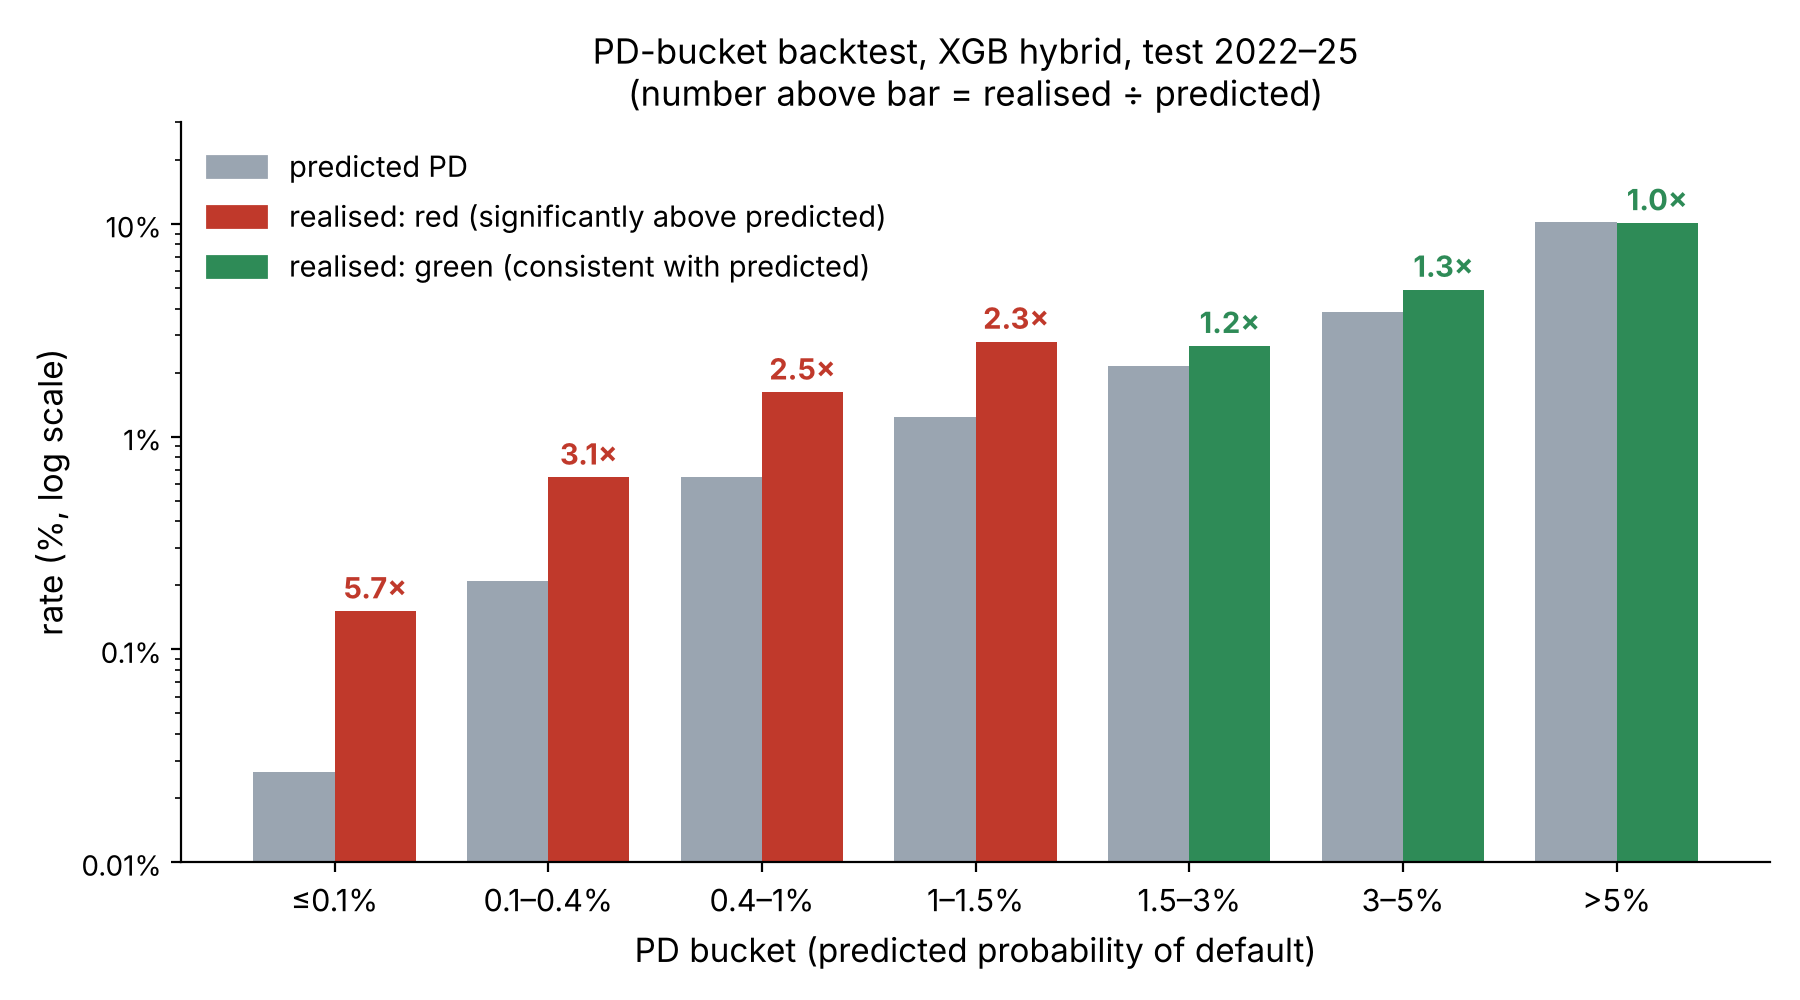
\includegraphics[height=5.6cm]{assets/06_pd_backtest.png}
\caption{Left: realised bankruptcy rate against mean predicted PD by decile (test set). Right: PD-bucket
backtest of the hybrid XGBoost; the number above each pair is realised $\div$ predicted.}
\label{fig:calibration}
\end{figure}

\paragraph{Firm size.} Small firms are hardest. By terciles of total assets, XGB-static reaches AUROC 0.770
(small), 0.874 (medium) and 0.919 (large); the structural model 0.759, 0.791 and 0.849. Small firms have noisier
statements and shorter histories, and the advantage of ML over the structural model is smallest there.

\subsection{Comparison with related work}

The trees-over-logit gain (+3.5 AUROC points [2.1, 4.7]) is close to the 2.6 points of~\cite{moscatelli2020}
on public data, although the country, target and period differ. As in~\cite{bharath2008}, DD is not
sufficient: ML beats it by 0.062. As in~\cite{campbell2008}, DD adds little next to accounting variables,
at least for flexible models. Unlike~\cite{pellegrino2024}, the LSTM does not beat trees once the trees
receive lag features; their data and split differ, so this is a consistent finding rather than a direct
replication.

\section{Conclusion and discussion}
\label{sec:conclusion}

\paragraph{Answers.} On public SEC data, the best bankruptcy model is a gradient-boosted tree with firm history
(AUROC 0.872 on 2022--2025, against 0.800 for the structural baseline).
\begin{description}
  \item[RQ1] Structural features help a linear model (+0.021 AUROC, significant) but add nothing measurable to
             tree models, which recover the same information from accounting ratios; the DD formula does not
             beat its raw inputs.
  \item[RQ2] New industry: a modest tilt towards the hybrids (4 of 6 industries). New period, new industry and period,
             and limited data: no reliable gain. Structure is relatively strongest at short horizons. H2's apparent
             edges are confounded with class weighting.
  \item[RQ3] The definition of the default point matters more than the drift; a liabilities-based point beats a debt-based one.
  \item[RQ4] History helps: hand-made lag features beat the LSTM, and structure adds nothing once history is included.
\end{description}
Merton structure remains a useful interpretable baseline and helps simple models, but is largely redundant for
flexible ones. The main contribution is the reproducible pipeline and the controlled comparison, not a new
state-of-the-art model.

\paragraph{What the evidence does not establish.} All results are associations in one market and period; they say
nothing causal about why firms fail. The negative RQ1 result is about \emph{our} price-free DD; a market-based DD
might behave differently. With about 200 bankrupt firms per test period, small differences cannot be resolved.

\paragraph{Limitations.}
\begin{itemize}
  \item \textbf{Label:} 8-K Item~1.03 is a disclosure proxy; out-of-court restructurings and firms that stop filing count as non-events.
  \item \textbf{Structural inputs:} book-value asset volatility and a stale annual public float are weaker than a daily market DD.
  \item \textbf{Coverage:} only standard XBRL tags; debt is missing in about half of the filings; 215 of the 993 bankrupt firms have no usable filings.
  \item \textbf{Calibration drift:} PDs calibrated on one calm year are too low in a stressed period.
  \item \textbf{Equal footing:} H2 is trained without class weights while the baselines use them.
\end{itemize}

\paragraph{Responsible use.} A PD model can affect who gets credit. SHAP values give feature-level explanations
for each prediction, which supports review by a credit analyst. The data contain no personal or protected
attributes, so a fairness analysis in the usual sense is not possible; the size results show that small firms
receive less accurate scores. The model should support human decisions, with PD levels recalibrated before use.

\paragraph{Next steps.} (1) Compare H2 with an \emph{unweighted} ML model in every regime, the one open question
that could change an answer. (2) Recalibrate PDs on a rolling window, or update the intercept to the current
bankruptcy rate. (3) Compute a true market DD from CRSP daily prices, including delisted firms, with our existing
solver. (4) Add text signals from 10-K filings, such as going-concern warnings.

\paragraph{Reproducibility.} The repository~\cite{repo} contains the SEC download scripts with hash manifests,
the label audit, the point-in-time panel builders and validator, the Merton toolbox, the evaluation package
(purged splits, all regimes, one training recipe for every model, firm bootstrap, PD backtest, unit tests), and the
notebook that writes every table and figure of this report (1--3 hours on a laptop CPU).


\section*{References}
\addcontentsline{toc}{section}{References}
\bibliographystyle{plain}
{\renewcommand{\section}[2]{}% the References heading above is kept from the template
\bibliography{references}}

\end{document}
